% Digital Logic Report Template
% Created: 2020-02-13 Sebastian Lopez, Megan Gordon, and Jane Ross  

%==========================================================
%=========== Document Setup  ==============================

% Formatting defined by class file
\documentclass[11pt]{article}

% ---- Document formatting ----
\usepackage[margin=1in]{geometry}	% Narrower margins
\usepackage{booktabs}				% Nice formatting of tables
\usepackage{graphicx}				% Ability to include graphics

%\setlength\parindent{0pt}	% Do not indent first line of paragraphs 
\usepackage[parfill]{parskip}		% Line space b/w paragraphs
%	parfill option prevents last line of pgrph from being fully justified

% Parskip package adds too much space around titles, fix with this
\RequirePackage{titlesec}
\titlespacing\section{0pt}{8pt plus 4pt minus 2pt}{3pt plus 2pt minus 2pt}
\titlespacing\subsection{0pt}{4pt plus 4pt minus 2pt}{-2pt plus 2pt minus 2pt}
\titlespacing\subsubsection{0pt}{2pt plus 4pt minus 2pt}{-6pt plus 2pt minus 2pt}

% ---- Hyperlinks ----
\usepackage[colorlinks=true,urlcolor=blue]{hyperref}	% For URL's. Automatically links internal references.

% ---- Code listings ----
\usepackage{listings} 					% Nice code layout and inclusion
\usepackage[usenames,dvipsnames]{xcolor}	% Colors (needs to be defined before using colors)

% Define custom colors for listings
\definecolor{listinggray}{gray}{0.98}		% Listings background color
\definecolor{rulegray}{gray}{0.7}			% Listings rule/frame color

% Style for Verilog
\lstdefinestyle{Verilog}{
	language=Verilog,					% Verilog
	backgroundcolor=\color{listinggray},	% light gray background
	rulecolor=\color{blue}, 			% blue frame lines
	frame=tb,							% lines above & below
	linewidth=\columnwidth, 			% set line width
	basicstyle=\small\ttfamily,	% basic font style that is used for the code	
	breaklines=true, 					% allow breaking across columns/pages
	tabsize=3,							% set tab size
	commentstyle=\color{gray},	% comments in italic 
	stringstyle=\upshape,				% strings are printed in normal font
	showspaces=false,					% don't underscore spaces
}

% How to use: \Verilog[listing_options]{file}
\newcommand{\Verilog}[2][]{%
	\lstinputlisting[style=Verilog,#1]{#2}
}




%======================================================
%=========== Body  ====================================
\begin{document}

\title{ELC 2137 Lab \#5: Intro to Verilog }
\author{Sebastian Lopez, Megan Gordon, and Jane Ross }

\maketitle


\section*{Summary}

In this lab we organized the files and adhered to the given folder structure. We had to learn the basic Verilog syntax and used it to create simple components and systems. We then created a full adder using both gate-level and functional/behavioral styles of coding. Following that we combined full adder components to create a 2-bit and 4-bit adder/subtractor. Throughout the process of the lab we also had to create test benches in order verify our designs.  

\section*{Q\&A}


\begin{enumerate}
	\item \textbf{Comment on whether the simulations match the expected output values.} 
		
	In last week's lab we found the expected output values using variables a, b, and mode. This week after testing and running the code, our simulations did match the results of the expected outcome.  
	
	\item \textbf{What is the one thing you still don't understand about Verilog?}
	
	We don't fully understand the conditions of the if statements. We are also not fully understanding the application of a proper 'always' statement. 
	 
\end{enumerate}

\section*{Results}

	- A very prominent error was that we could not seem to find the correct path for our 'out' variable in the sseg1.sv file.  
	- We then figured out that our statements in the sseg1test.sv were incorrect. Instead of repeating the same statements we did in the source code file, we decided it would be right 
	      to make an exclusive statement for all values of sw, and an.
	- 
\section*{Code}
	
\begin{lstlisting}[style=Verilog,
caption=mux2_4b Source Code,
label=mux2_4b:ex
]
`timescale 1ns / 1ps

module mux2_4b(
input [3:0] in0, in1, 
input sel, 
output [3:0] out
); 

assign out = sel? in0:in1; 

endmodule //mux2_4b
\end{lstlisting}

\begin{lstlisting}[style=Verilog,
caption=mux2_4b Test Code,
label=mux2_4b_test:ex
]
`timescale 1ns / 1ps
// ELC 2137 - Lab6 - 02/20/2020
// Sebastian Lopez and Megan Gordon

module mux2_4b_test( );

reg [3:0] in0, in1;
reg sel; 
wire [3:0] out;

mux2_4b Test1(
.in0(in0), .in1(in1), .sel(sel),
.out(out)
); 

initial 
begin

sel = 1;
in0 = 0;
in1 = 1;
#10;  
sel = 1; 
in0 = 1; 
in1 = 0; 
#10; 
sel = 0;
in0 = 0;
in1 = 1;
#10;  
sel = 0; 
in0 = 1; 
in1 = 0; 
#10; 
$finish;

end  

endmodule//mux2_4b_test
\end{lstlisting}

\begin{lstlisting}[style=Verilog,
caption=Sseg Decoder Source Code,
label=sseg_decoder:ex
]
`timescale 1ns / 1ps
// ELC 2137 - Lab6 - 02/20/2020
// Sebastian Lopez and Megan Gordon

module sseg_decoder(
input [3:0] num,
output reg [6:0] sseg 
);

always @* 
case (num) 
4'h0: sseg = 7'b1000000;
4'h1: sseg = 7'b1111001;
4'h2: sseg = 7'b0100100;
4'h3: sseg = 7'b0110000;
4'h4: sseg = 7'b0011001;
4'h5: sseg = 7'b0010010;
4'h6: sseg = 7'b0000010;
4'h7: sseg = 7'b1111000;
4'h8: sseg = 7'b0000000;
4'h9: sseg = 7'b0010000;
4'hA: sseg = 7'b0001000;
4'hb: sseg = 7'b0000011;
4'hC: sseg = 7'b1000110;
4'hd: sseg = 7'b0100001;
4'hE: sseg = 7'b0000110;
4'hF: sseg = 7'b0001110;
endcase 
endmodule //sseg_decoder
\end{lstlisting}

\begin{lstlisting}[style=Verilog,
caption=Ssed Decoder Test Bench Code,
label=ssed_decoder_test:ex
]
`timescale 1ns / 1ps
// ELC 2137 - Lab6 - 02/20/2020
// Sebastian Lopez and Megan GordonS

module sseg_decoder_test();

reg [3:0] num; 
wire [6:0] sseg; 

integer i; 

sseg_decoder d1(
.num(num),
.sseg(sseg)
);  

initial begin 
for (i = 0; i <=8'hF; i=i+1) begin 
num = i; 
#10; 
end 
$finish; 
end 
endmodule //sseg_decoder_test
\end{lstlisting}

\begin{lstlisting}[style=Verilog,
caption=Sseg1 Source Code,
label=sseg1:ex
]
`timescale 1ns / 1ps
// ELC 2137 - Lab6 - 02/20/2020
// Sebastian Lopez and Megan Gordon

module sseg1(
input [15:0] sw, //switches 
output [3:0] an, // 7-segment digits
output [6:0] seg, // 7-seg segments
output dp // decimal point 
);

wire [3:0] out; 

not not1(an[1],sw[15]);
assign an[0] = sw[15];
assign an[3:2] = 3;
assign dp = 1; 

mux2_4b mux1(
.in0(sw[3:0]), .in1(sw[7:4]), .sel(sw[15]), 
.out(out) 
);

sseg_decoder sseg2(
.num(out),
.sseg(seg)
); 

endmodule //seg1
\end{lstlisting}

\begin{lstlisting}[style=Verilog,
caption=Sseg1 Test Bench Code,
label=sseg1_test:ex
]
`timescale 1ns / 1ps
// ELC 2137 - Lab6 - 02/20/2020
// Sebastian Lopez and Megan Gordon

module sseg1(
input [15:0] sw, //switches 
output [3:0] an, // 7-segment digits
output [6:0] seg, // 7-seg segments
output dp // decimal point 
);

wire [3:0] out; 

not not1(an[1],sw[15]);
assign an[0] = sw[15];
assign an[3:2] = 3;
assign dp = 1; 

mux2_4b mux1(
.in0(sw[3:0]), .in1(sw[7:4]), .sel(sw[15]), 
.out(out) 
);

sseg_decoder sseg2(
.num(out),
.sseg(seg)
); 

endmodule //seg1
\end{lstlisting}

\begin{figure}[ht]\centering
	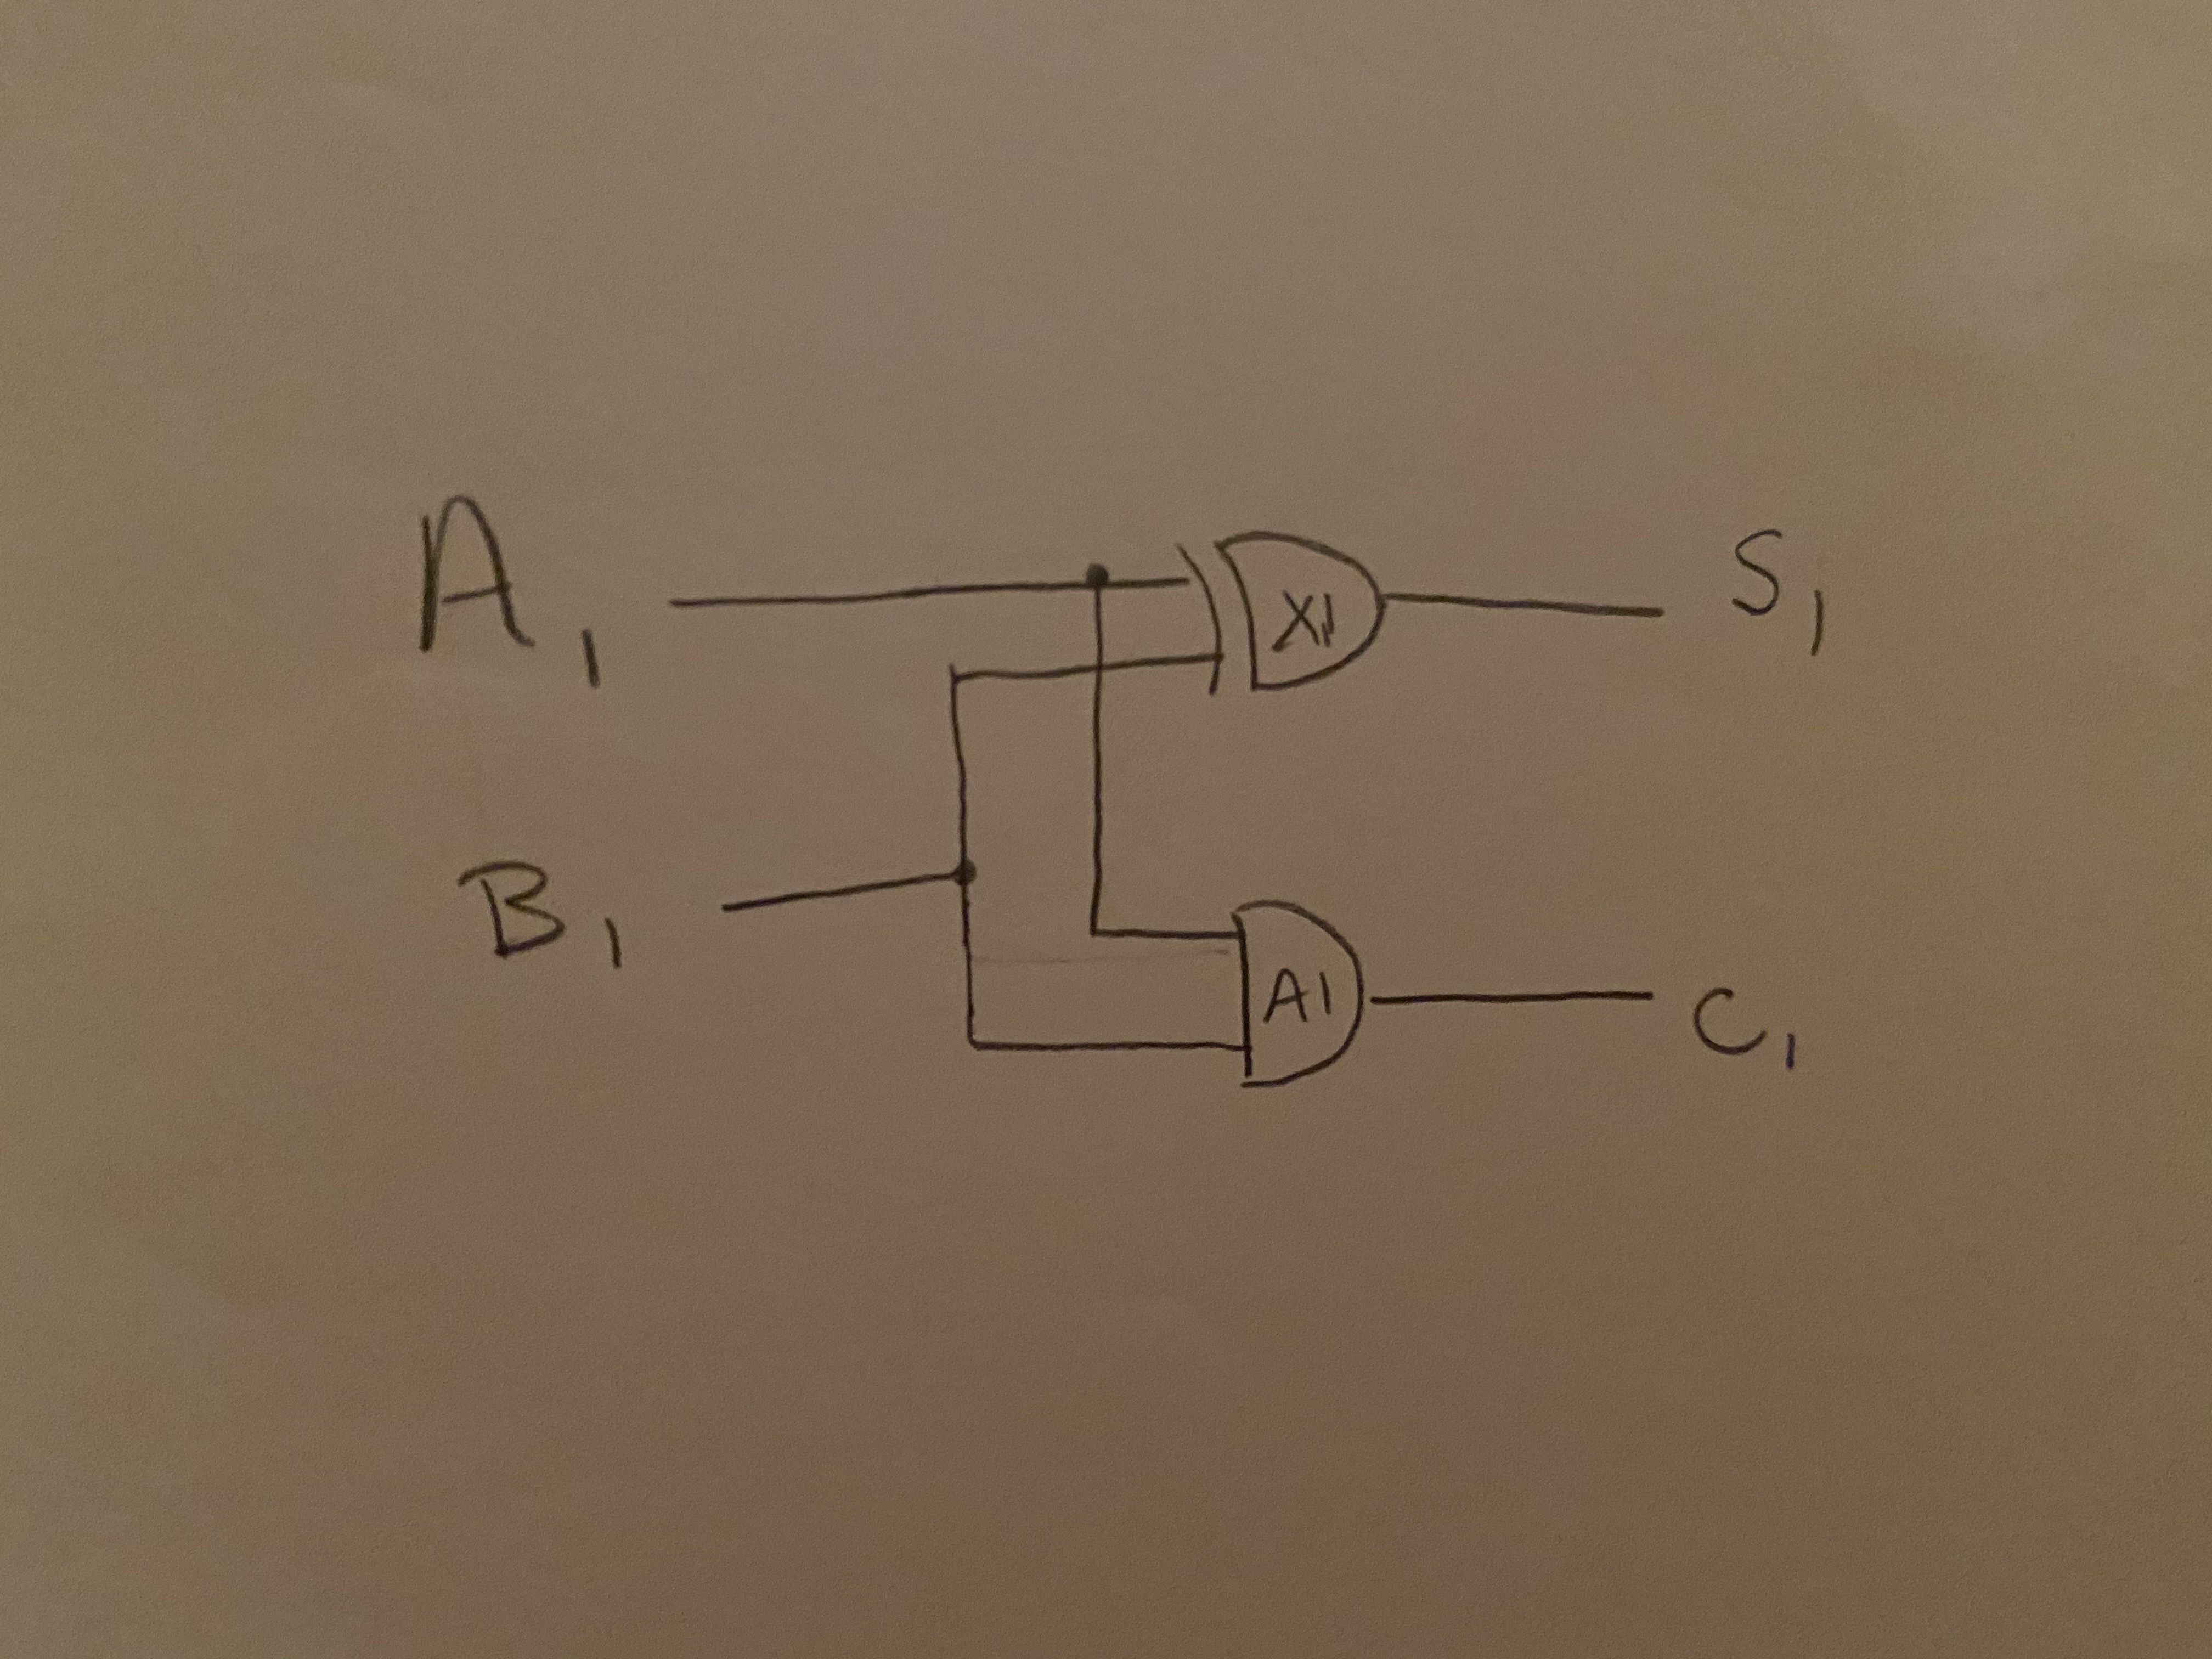
\includegraphics[width=0.6\textwidth, trim=10cm 10cm 10cm 10cm,clip]{Half-Adder Lab05}
	\caption{This is the diagram for the Half Adder}
	\label{fig:Half-Adder}	
\end{figure}

\begin{figure}[ht]\centering
	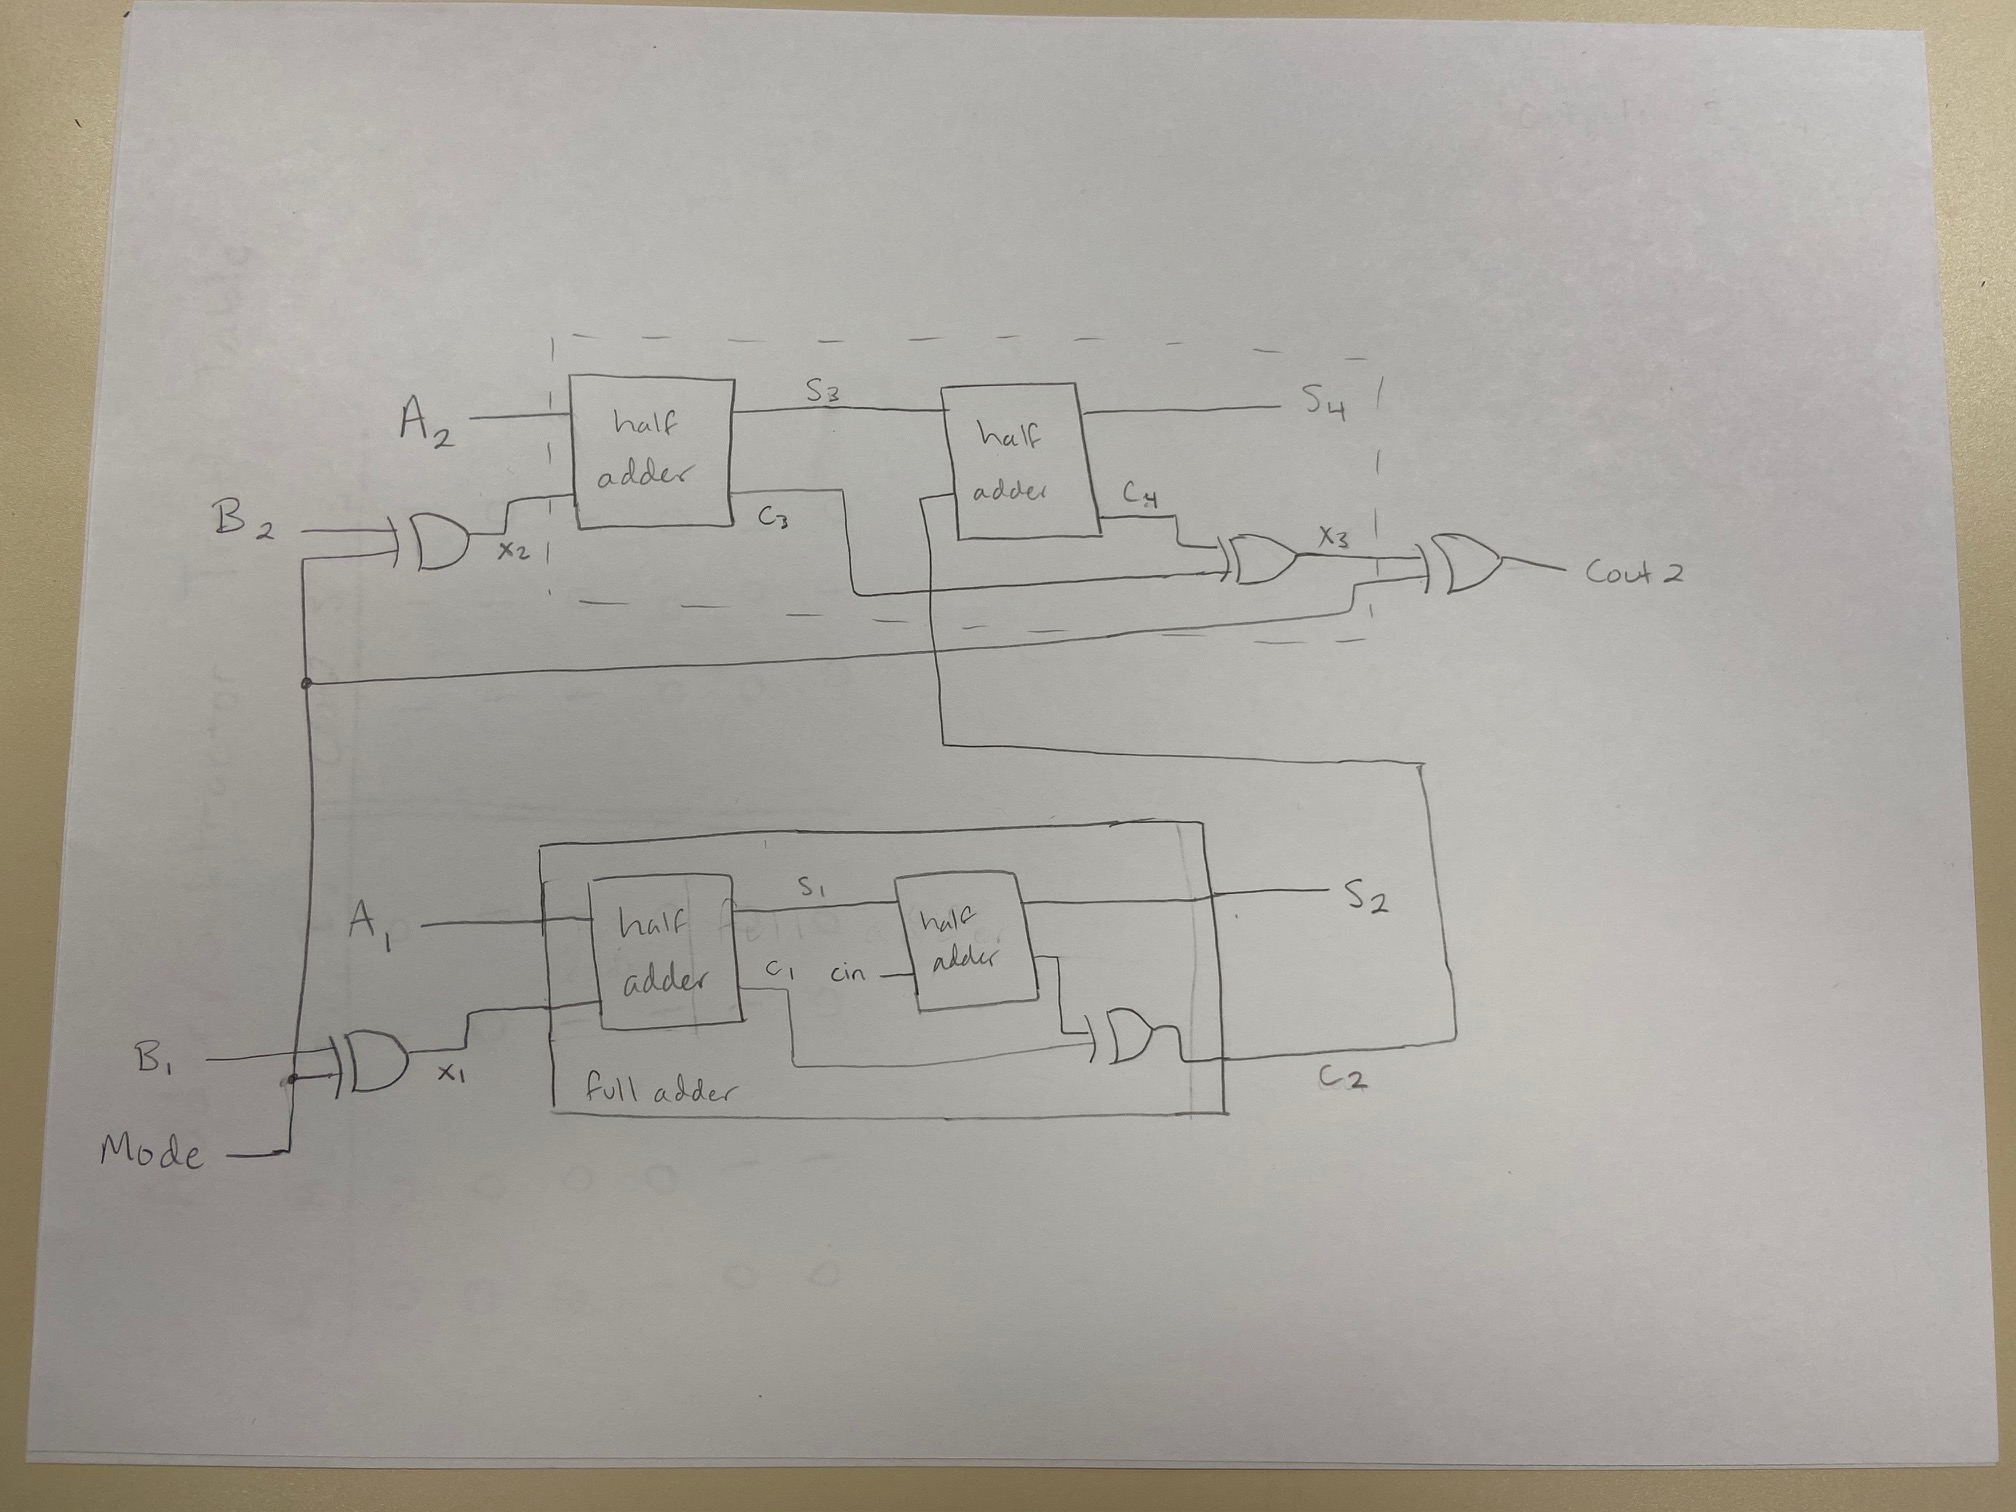
\includegraphics[width=0.6\textwidth, trim=3cm 10cm 10cm 10cm,clip]{2-bit Adder Lab05}
	\caption{This is the diagram for the Full and 2-bit Adder}
	\label{fig:Full_2-bit_Adder}	
\end{figure}

	\item ERTs and screenshots for Behavioral Simulations 
	
\begin{table}[ht]\centering
	\caption{Half Adder ERT}
	\label{tbl:Half_Adder_ERT}
	\begin{tabular}{c||cc|cc}
		\toprule
		Time (ns) & A1 & B1 & C1 & S1\\
		\midrule
		0 & 0 & 1 & 0 & 1\\
		10 & 0 & 0 & 1 & 1\\
		20 & 0 & 0 & 0 & 1\\
		30 & 0 & 1 & 1 & 0\\
		\bottomrule
	\end{tabular} 
\end{table} 

\begin{table}[ht]\centering
	\caption{Full Adder ERT}
	\label{tbl:Half_Adder_ERT}
	\begin{tabular}{c||ccc|cc}
		\toprule
		Time (ns) & A1 & B1 & Cin & Cout & S\\
		\midrule
		0 & 0 & 0 & 0 & 0 & 0\\
		10 & 1 & 0 & 0 & 0 & 1\\
		20 & 1 & 1 & 0 & 1 & 0\\
		30 & 0 & 0 & 1 & 0 & 1\\
		40 & 1 & 0 & 1 & 1 & 0\\
		50 & 1 & 1 & 1 & 1 & 1\\
		\bottomrule
	\end{tabular} 
\end{table} 

\begin{table}[ht]\centering
	\caption{Full Adder ERT}
	\label{tbl:Half_Adder_ERT}
	\begin{tabular}{c||ccccc|ccc}
		\toprule
		Time (ns) & A1 & B1 & A2 & B2 & Mode & Cout & S2 & S4\\
		\midrule
		0 & 0 & 0 & 0 & 0 & 0 & 0 & 0 & 0\\
		10 & 0 & 1 & 0 & 0 & 1 & 1 & 1 & 1\\
		20 & 0 & 0 & 0 & 1 & 1 & 1 & 1 & 0\\
		30 & 0 & 1 & 0 & 1 & 1 & 1 & 0 & 1\\
		40 & 1 & 1 & 0 & 0 & 0 & 0 & 0 & 0\\
		50 & 0 & 1 & 1 & 0 & 0 & 0 & 0 & 1\\
		60 & 0 & 0 & 1 & 0 & 0 & 0 & 1 & 0\\	
		\bottomrule
	\end{tabular} 
\end{table} 

	
\begin{figure}[ht]\centering
	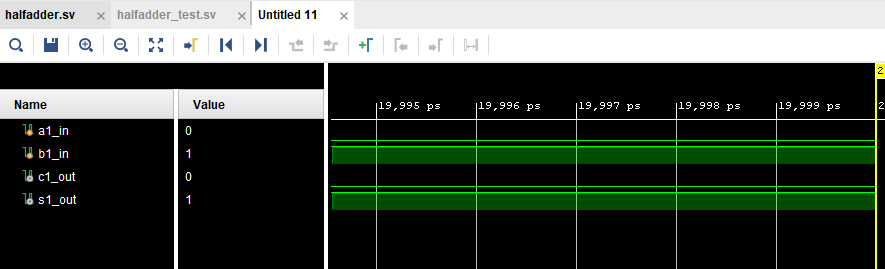
\includegraphics[width=0.75\textwidth]{Half Adder Simulation}
	\caption{This is the Half Adder Simulation Screenshot.}
	\label{fig:half_adder_sim}	
\end{figure}

\begin{figure}[ht]\centering
	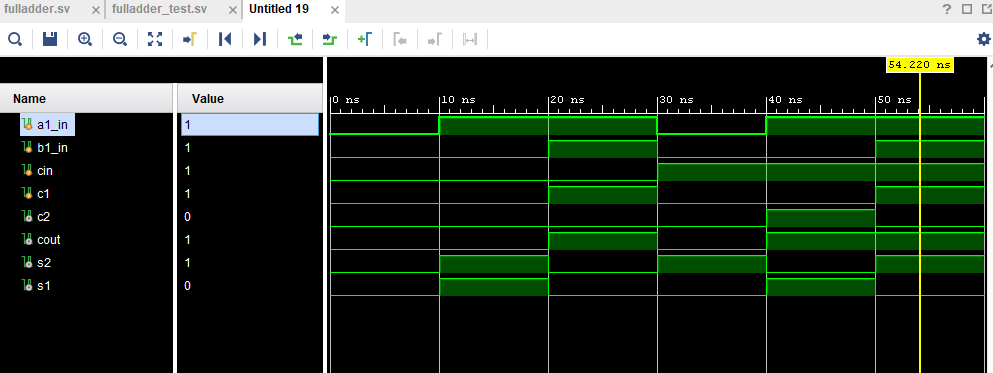
\includegraphics[width=0.75\textwidth]{Full Adder Simulation}
	\caption{This is the Full Adder Simulation Screenshot.}
	\label{fig:full_adder_sim}	
\end{figure}

\end{document}
